\documentclass{article}

\usepackage[top=2.5cm,left=2.5cm,right=2.5cm,bottom=2.5cm]{geometry}
\usepackage[utf8]{inputenc}
\usepackage[T1]{fontenc}
\usepackage[french]{babel}
\usepackage{graphicx}
\usepackage{pdflscape}

\title{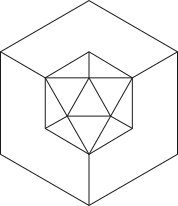
\includegraphics{logo.png}\vspace{2cm}\\Stage chez Let There Be Light \\ \large Rapport d'étonnement Exia A4}
\date{23 Janvier 2018}
\author{Stagiaire : Baptiste \bsc{Saclier} \\ Maître de stage : Benjamin \basc{Petit}\\Pilote de fromation : Julio \basc{Santilario}}

\begin{document}

\maketitle

\clearpage

\tableofcontents

\section{Introduction}

%TODO introduction

\clearpage

\section{Let There Be Light}

La société Let There Be Light (ou LTBL) est un société qui réalise des dispositifs interactifs pour pour l'événementtiel, la communication et la culture.
Elle fut fondée en 2014 par Benjamin \bsc{Petit} et Antoine \bsc{Vanel} sous le nom de Beam'Art.
En 2016, elle change de nom et de status pour devenir l'entreprise que l'on connait actuellement.
Aujourd'hui Mr \bsc{Petit} en est le seul dirigeant.

\begin{description}
    \item[2012] Première fêtes des lumières dans le cadre d'une association avec un spéctacle intéractif nommé "Hypermétrope"
    \item[2014] Fondation de la société Beam'Art
    \item[2014] Installation intéractive "Hi Striker" sur le palais de justice
    \item[2014] Mapping "TranJS" à Bernes
    \item[2015] Installation intéractive "Lumibus" pour Keolis
    \item[2016] Changement de nom pour devenir Let There Be Light
    \item[2016] Participation à la création du showroom Pavillon de l'innovation pour Michelin
    \item[2017] Scenographie au Transbordeurs "DELete"
\end{description}

\subsection{Structure}

Let There Be Light est, sur la majorité des projets, un partenaire de la société Vendredi 4.
Vendredi 4 est une société de communication spécialisée dans l'interaction.
Elle délegue le travail de développement à LTBL sur la majorité de ses projets.
Les contrats sont obtenus par Sylvie \bsc{Madamour}, la charte graphique du projet est alors composée par Vendredi 4.
LTBL intervient sur l'intégration de cette charte graphique dans des installations intéractives dans des salons au des showrooms.

Les équipes de Vendredi 4 et de LTBL sont assez réduite.
L'éfféctif de Vednredi 4 est donc de 3 employés quand LTBL compte un employé (Mr \bsc{Petit}) et un prestataire (Mr \bsc{Limoge})

\begin{figure}[h]
    \centering
    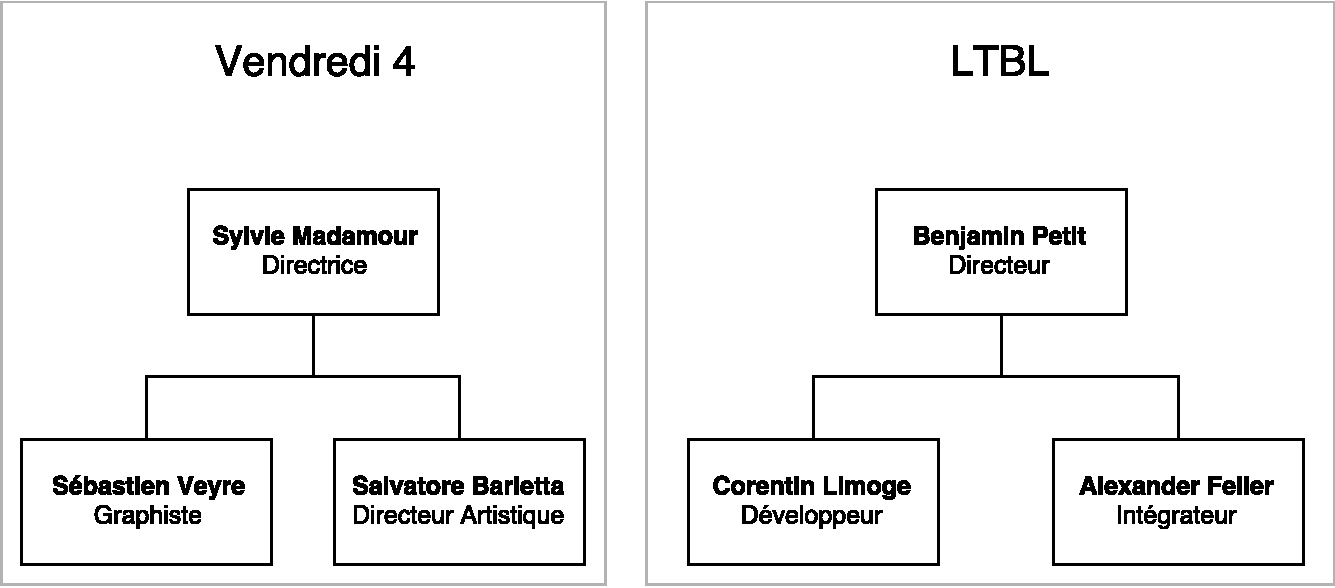
\includegraphics[scale=0.7]{Structure-LTBL.pdf}
    \caption{Structure de LTBL et Vendredi 4}
\end{figure}

Les deux entreprises sont trés liés, elles partagent les même locaux et communiqument beaucoup ensemble sur les projets en cours et à venir.

On retrouve alors Benjamin \bsc{Petit}, le gérant, et Corentin \bsc{Limoge} du coté LTBL.
Benjamin s'occupe des conseils et de la gestion de l'entreprise.
Il s'occupe aussi de l'aspect technique des installations par le choix des technologies de pointage et d'affichage.
Corentin est employé par LTBL mais dispose d'un status d'auto-entrepreuneur, on peut alors le considèrer comme un consultant.
Corentin est en charge du développement des applications qui seront éxécutés sur les installations.

Du coté Vendredi 4 on retrouve Sylvie \bsc{Madamour}, la directrice, Salvatore \bsc{Barletta}, directeur artistique, et Sébastien \bsc{Veyre}, graphiste.
Sylvie est en charge des contrats, devis et de la communication avec les clients.
Salvatore est directeur artistique chez vendredi 4, il s'occupe de concevoir et présenter les design des installations aux clients.
Sébastien est graphiste et est en charge de représenter les futurs interfaces des installations mais aussi de travailler sur des rendus en Motion Design pour donner un premier aperçu de la futur application pour les clients et les intégrateurs.

\subsection{Projets}

Les deux entrprises travailleur ensemble pour proposer des services suivants :

\begin{itemize}
    \item Conseils téchniques
    \item Conseils en intéraction
    \item Design graphique
    \item Développement d'applications intéractives
    \item Installations
\end{itemize}

Ainsi, les deux entreprises peuvent suivre la production d'une application intractive de sa conception jusuqu'a son installation.

\medskip

Les projets suivi par LTBL sont les suivants :

\paragraph{Dispositifs de présentation intéractifs} Le plus souvent utilisés dans les salons et showrooms, les dispositifs intéractifs permettent une présentation des produits de manière ésthétique.
L'objectif de LTBL est donc de concevoir cette installation.
Cela passe par la conception du système phisique est des composants requis maus aussi par la conception et le développement de l'interface utilisateur qui doit être réactive et esthetique.
La majorité de ce type de projet est la présentation d'informations sur un produit sur un écran tactile sous forme de table tactile.

\paragraph{Vidéo Mapping} Le plus souvent présenté lors d'événements, le vidéo mapping consiste en la projection d'une image déformée sur une structure pouavnt être un batiment ou une installation spécifique.
Cette image utilise une représentation de la structure pour se déformer et épouser sa forme lors de la projection.
Ce type d'installation permet, au travers de jeux de lumière et d'illusions, de donner vie a la structure ou au batiment.
On retrouve ce type d'installation à la fête des lumières de Lyon par exemple.

\paragraph{Conseils technique ou en interaction} Fort de son experiance dans le domaine de l'intéractivité, LTBL peut aussi donner des conseils en interactivité dans le cadre de projets cités plus haut.

\paragraph{Fête des lumières} La fêtes des lumières est une manifestation Lyonnaise prenant place aux endroits importants de la ville.
Cette fête met en lumière de nombreuses installations lumineuses et intéractives.
Chaque année, LTBL peut proposer un projet d'installation en rapport avec un batiment de la ville sur lequel s'installer.
Ce projet est alors évalué et est accepté ou non en fonction de la faisabilité, l'esthetique et le cout de l'installation.
La dernière fête des lumière a laquelle a participé LTBL fut celle de 2015 avec une installation nommée "Lumibus".
Cette installation présentait un Bus munis de panneaux LED régissant aux accelerations su bus.
Les années précédentes, LTBL à aussi présenté Hi Striker, une installation reprenant le jeu de foire de la massue ou les participants doivent Tapper le plus fort possible sur un capteur à l'aide d'une massue.
Plus la frappe est forte plus le batiment s'illumine.
Cette installation se trouveait au palais de justice.
Plus récemment, LTBL à participé à la fête des lumières de Hong Kong avec un projet reprenant le même principe mais en animant un dragon.

\begin{figure}[h]
    \centering
    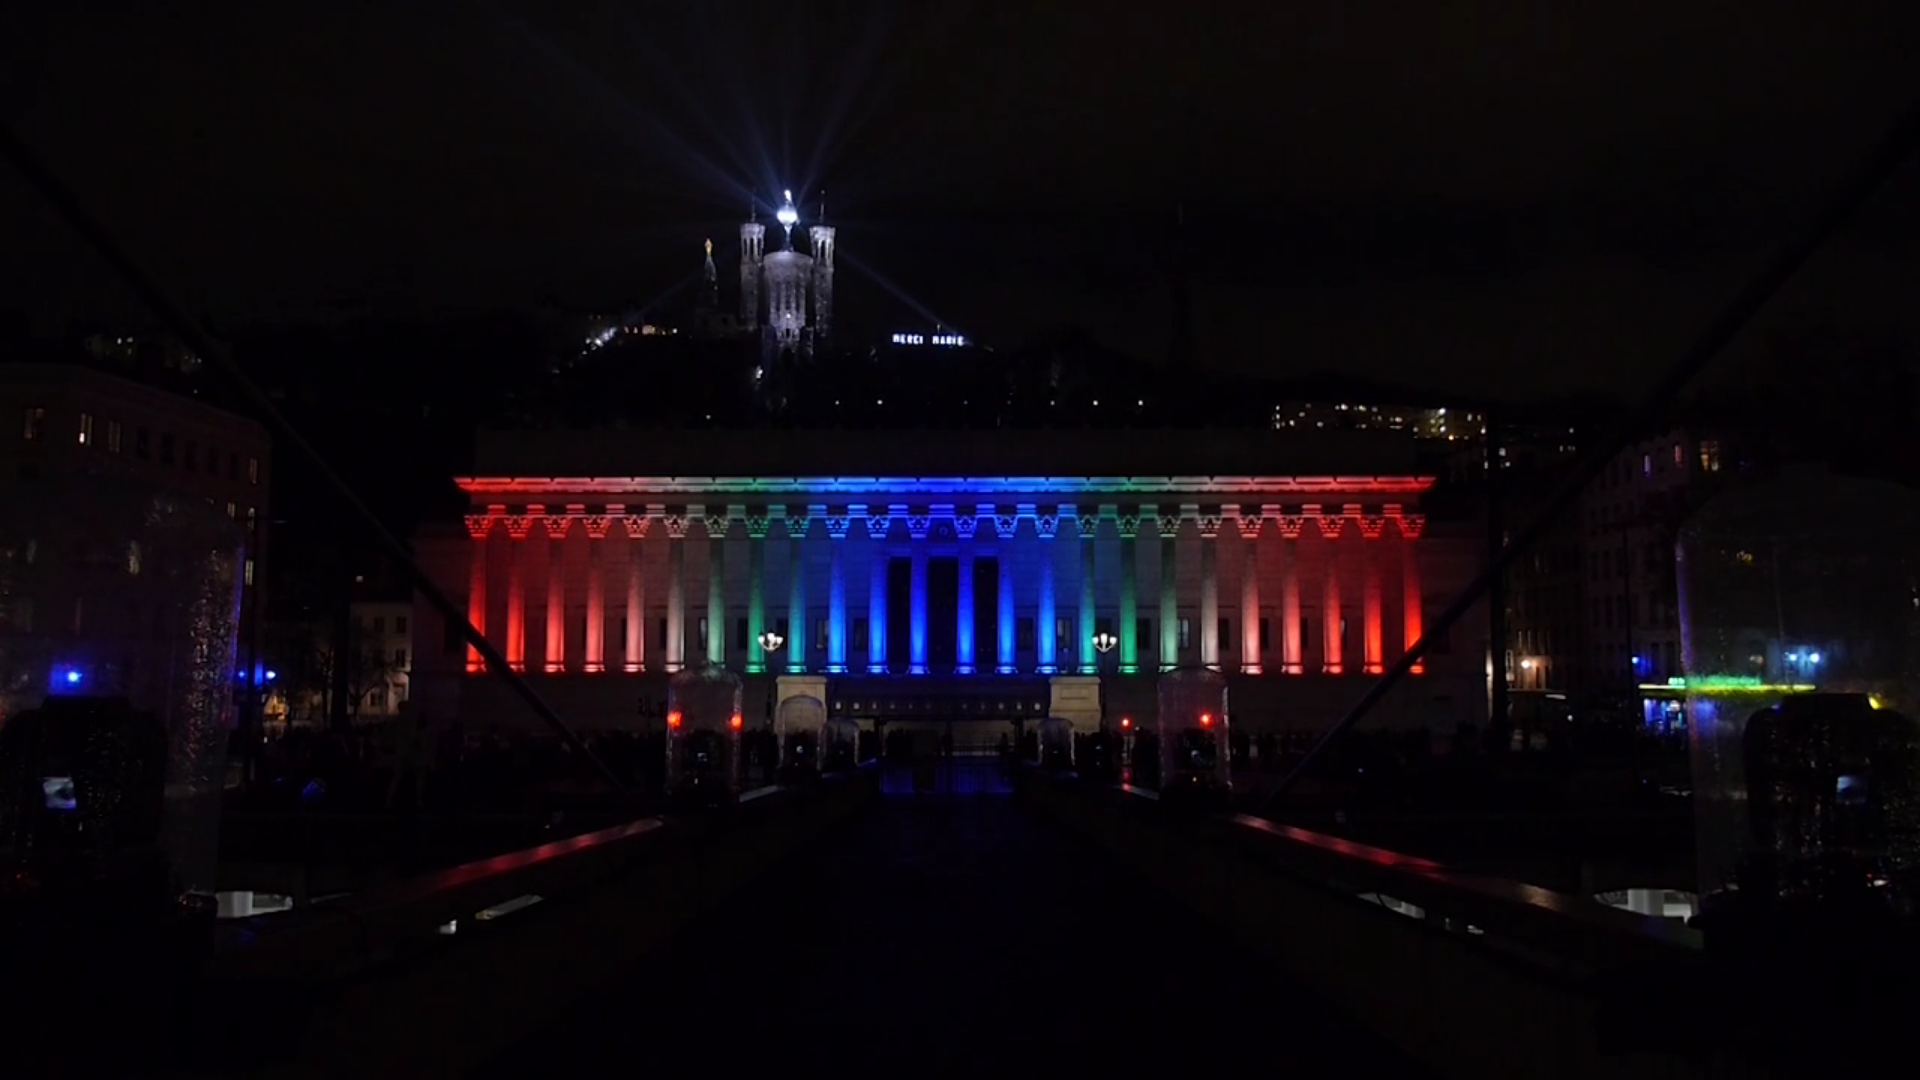
\includegraphics[scale=0.2]{hi-striker.png}
    \caption{L'installations "Hi Striker" à la Fête des lumières de Lyon}
\end{figure}


\begin{figure}[h]
    \centering
    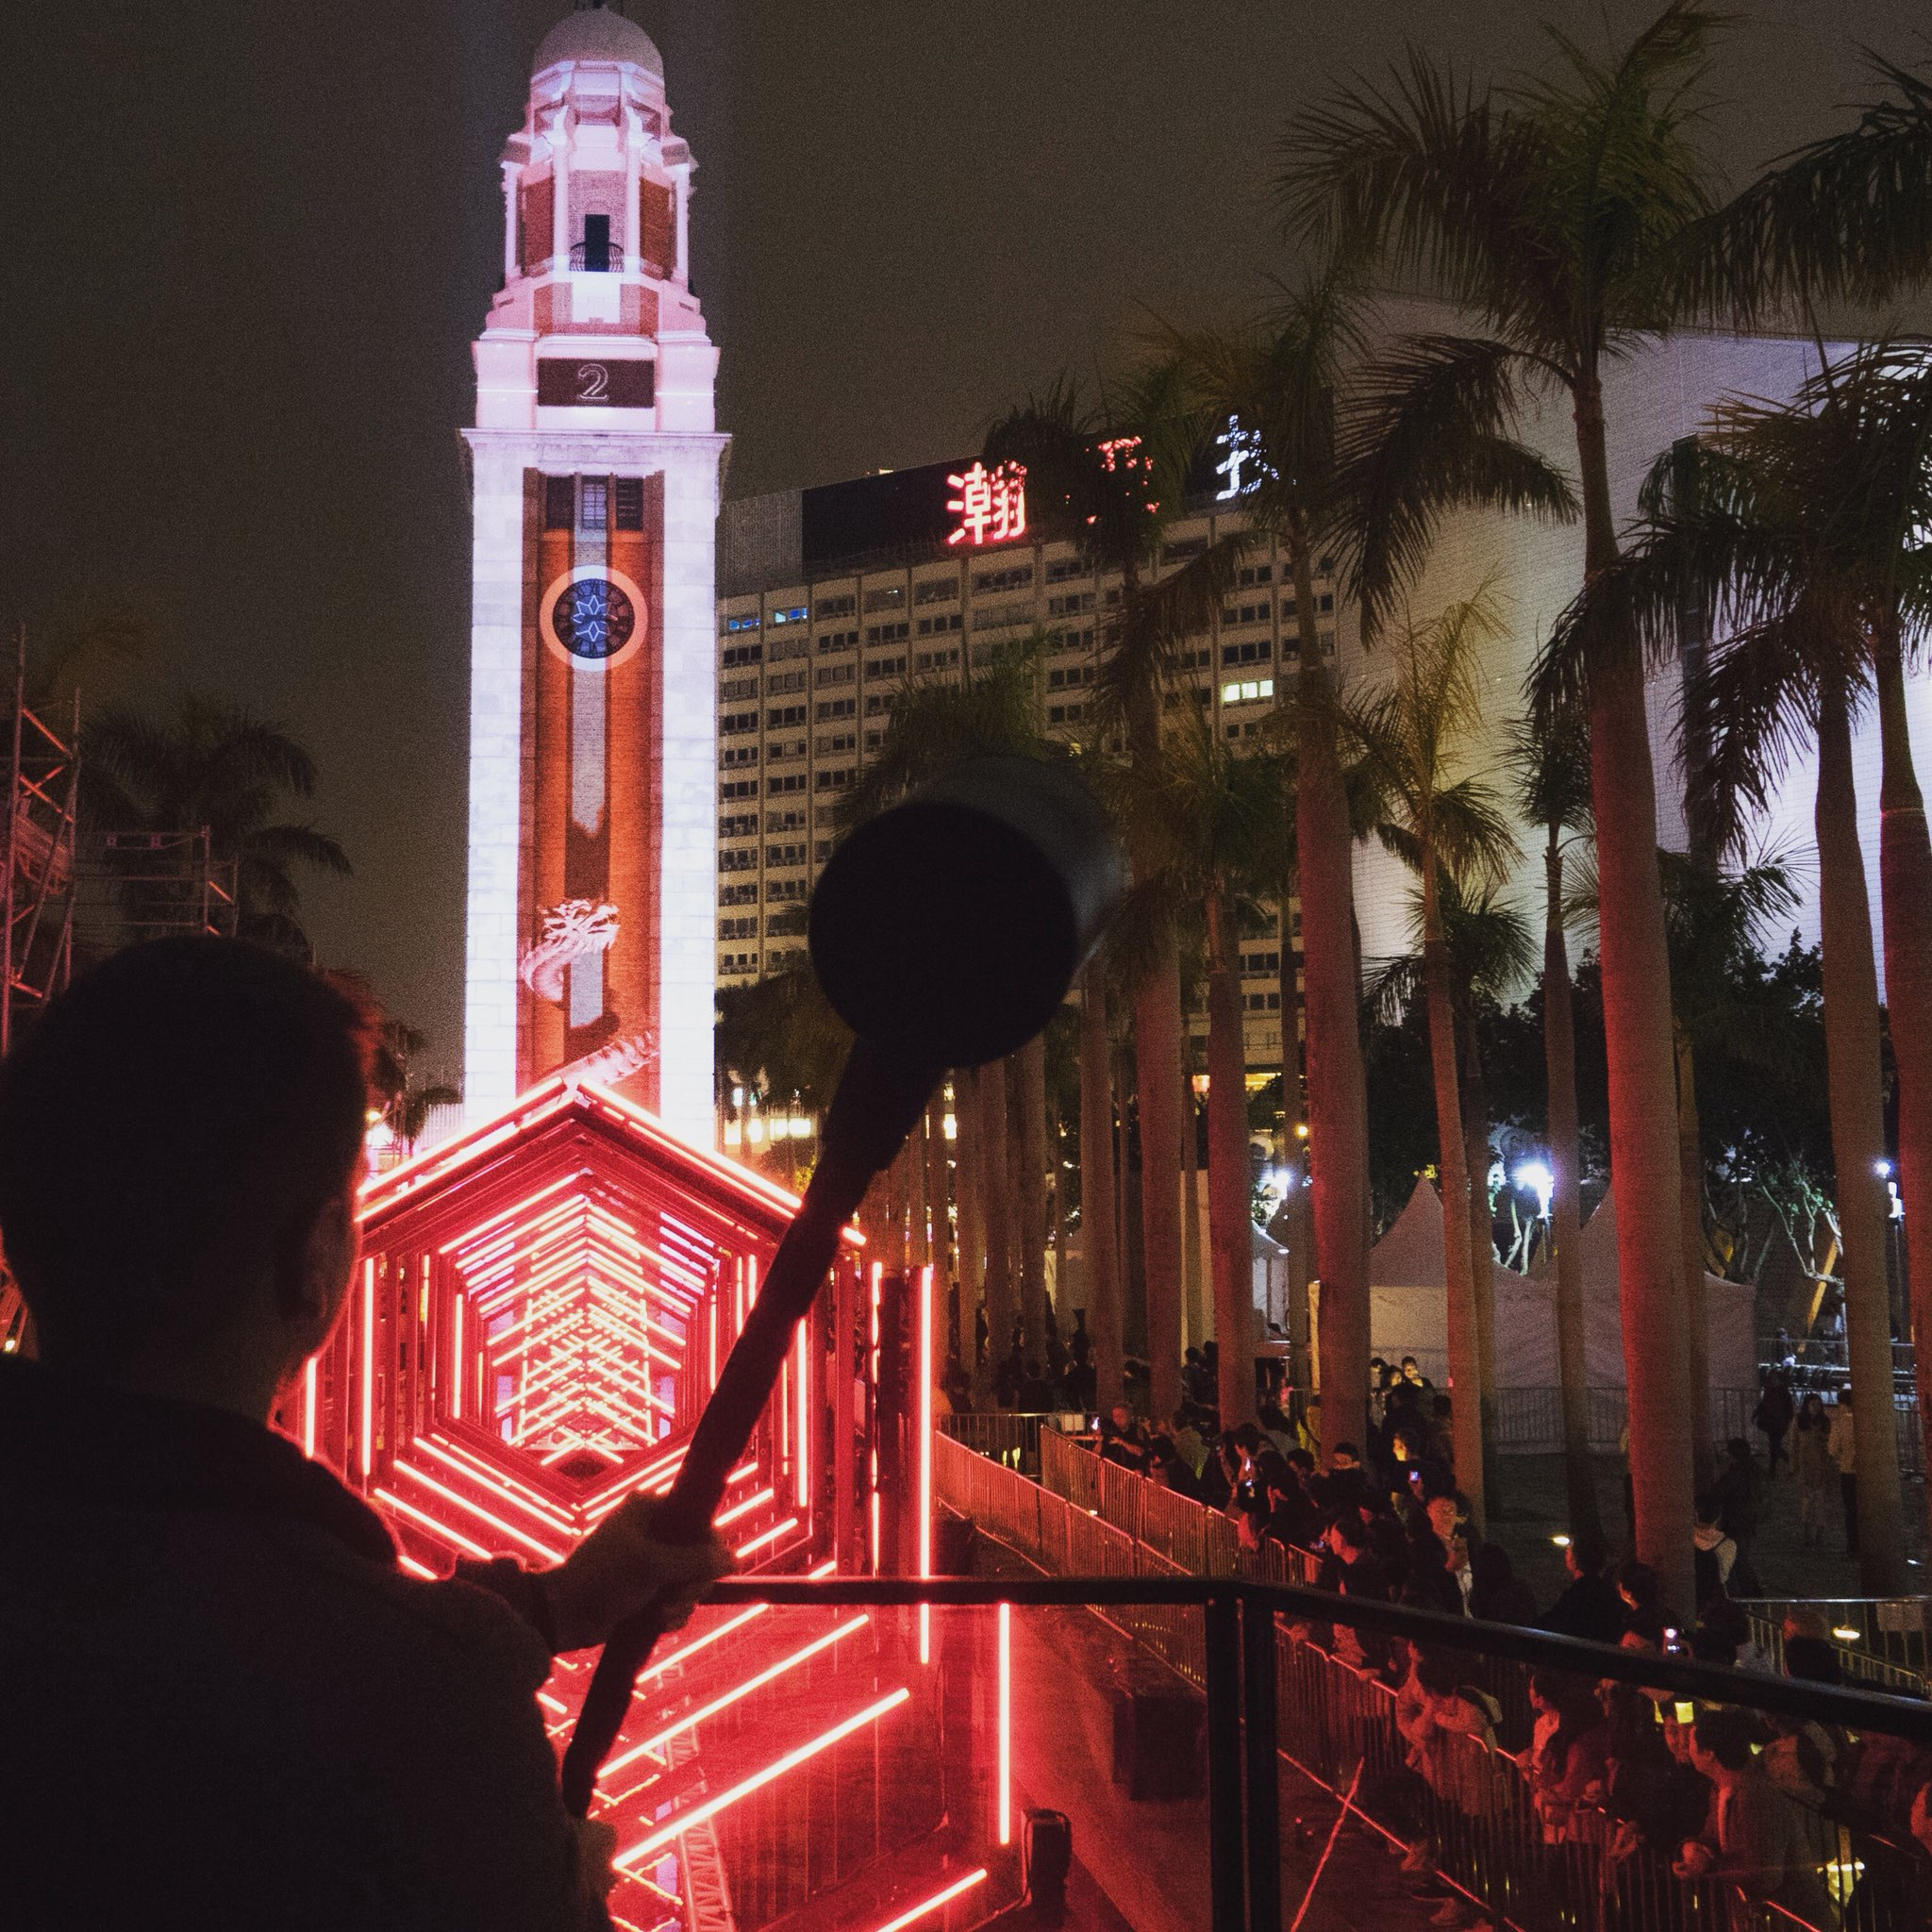
\includegraphics[scale=0.1]{long-striker.jpg}
    \caption{L'installation "Long Striker" à la fête des lumières de Hong Kong}
\end{figure}

\clearpage

\subsubsection{Clients}

Les clients de LTBL et de Vendredi 4 sont, le plus souvent, de la région rhône alpes mais peuvent aussi être en région parisienne.
Ces clients sont des PME ou des grands groupes désirant de nouvelles installations intéractives pour leurs showrooms.
Au travers de ces installations, ils peuvent montrer leur produit de manière esthétiques à leurs clients.
Les showrooms ne sont pas les seuls installations organisés par LTBL, on retrouve aussi des présentation de produits pour les salons ou l'affichage de données pour la productivité.

\medskip

Quelques clients :

\begin{itemize}
    \item Biomérieux
    \item EDF
    \item Michelin
    \item Somfy
    \item Visiativ
    \item Courchevel
    \item Fête des lumières
    \item Et bien d'autres \ldots
\end{itemize}

\section{Intégration}

Mon intégration dans l'entrprise c'est faite tres rapidement.

J'ai commencé par passer l'entretien le 27 Novembre qui c'est très bien passé.
J'ai découvert une équipe de 2 personnes sympatiques et ayant des projets intéressants.
On m'a informé sur les objectifs de mon stage.

J'ai intégré l'entreprise le 9 Janvier.
J'ai alors découvert ma première mission, le développement d'une application Electron pour afficher les produits de l'entreprise Biomérieux.

La première journée fut une journée de mise en place ou j'ai pu acceder aux infrastructure de LTBL.
J'ai eu acces à leur dépot de code sur BitBucket et les conversations de groupe de LTBL et Vendredi 4 sur Slack.
Enfin, j'ai pu me joindre au Trello mis en place pour le projet que j'ai à faire.

Durant ma première semaine, je me suis familiarisé avec ma première mission et les technologies qui l'entourent comme Electron et les WebComponents.
Je conaissait déjà Electron, une solution de développement d'application natives avec des outils Web.
En revanche je ne connaissait pas les Webcomponents, un nouveau standard web permettant de concevoir des tags HTML personnalisés.
Par contre, j'avais déjà utilisé des framework Javascript avec la même philosophie comme VueJS et Angular;
Avec ces compétences que je possèdait déjà et l'expériance de Corentin, j'ai pu apprendre ce nouveau système en une journée.

Le début de ma mission fut assez difficile car, même si je comprenait les bjectifs, aucun cahier des charges n'a formellement été rédigé.
Je me suis donc appuyé sur la vidéo en Motion Design de Sébastien pour en déduir les fonctionnalités à implémenter.
De plus, mon maitre de stage étant aux Etats unis pour le CES de Las Vegas, je ne pouvait pas lui parler sur mes horaires de travail ce qui rend la conception de la solution difficile.

En conclusion, les premières semaines de mon stage se sont très bien passé et je me suis intégré dans cette entreprise plus rapidement que dans les autres stages que j'ai éfféctué.
Cela est surement due à l'ambiance bonne enfant et sympatique des équipes et aussi de l'éfféctif réduit.

\section{Etonnement}

Durant les premières semaines de mon stage j'ai eu l'occasion de découvrir cette entreprise et ses particularités par rapport aux autres entreprises que j'ai intégré.

\paragraph{Ambiance} L'éfféctif réduit de l'etreprise (2 chez LTBL et 3 chez Vendredi 4) permettent de s'intègrer très facilement a l'équipe et de communiquer plus aisément.
Il n'est même plus nécéssaire d'utiliser le Slack mis en place pour communiquer sur les projets sur les heures de travail.
De plus, les employés de l'entreprises sont passionnés par leur domaine et cela se sent.
Ils sont très qualifiés et curieux dans la technologie et m'on déjà fait découvrir de nombreuses choses.
Enfin, la curiosité de l'équipe les amènent a découvrir de nouvelles technologies même si cela n'est pas l'objectif premier du projet.
Par exemple, l'entreprise à investi dans une imprimante 3D pour éxpérimenter cette technologie pouvant être utilise pour la fabrication de structure ou de boitier.

\paragraph{Deadlines} J'ai remarqué que LTBL est en charge de courts voir tres courts projets qui ne sont pas maintenus sur le long terme.
Ma première mission est un projet de développement d'application sunr un seul mois.
En effet, la première présentation du produit s'éfféctuera le 7 février.
La faible maintenance des projets de LTBL est justifiée par le fait qu'ils contrôlent leurs installations du hardware jusqu'au software par le choix des technologies a utiliser et l'installation chez le client.
Ainsi, une fois que l'installation fonctionne, il n'est plus nécéssaire de s'en occuper pour qu'elle fonctionne pendant plusieurs mois voir années.

\paragraph{Locaux \& matériel} Les locaux de LTBL sont assez petit et sont partagés par les deux entreprises.
Ces locaux sont composés de 2 bureaux, une salle principale avec mezzanine et une salle de pause.
Cela suffit pour les équipes mais la periode à laquelle je suis arrivée est un periode de livraison pour des projets de tables tactiles.
Ainsi, des écrans tactile de grande taille on été livrés pour pouvoir tester en conditions réel les applications.
De plus, au retour de la fète des lumières de Hong Kong, beaucoup de materiel comme des barres de LED et des vidéosprojecteurs ont été stockés dans les locaux.

\paragraph{Cahier des charges} %TODO Pas de cahier des charges rédigé ?

\section{Missions}

Durant mon entretien, on m'a informé des technologies utilisées par l'entreprise dans les différents projets mis en place.
On retrouve \emph{Open frameworks}, un ensemble de librairies en C++ permettant la creation d'applications interactives.
L'entreprise utilise aussi beaucoup \emph{Electron}, une librairie permettant de concevoir des applications native a l'aide des technologies Web.
Electron est très utilisé dans la creation d'interface car les langages web sont concus dans cet optique.
De plus, Electron disposant du moteur de rendu Web de Chrome, il est possible d'utiliser des technologies récentes comme les Webcomponents\footnote{Les webcomponents sont des éléments HTML personnalisés crés par le développeur. Ils diposent de leur propre style et de leur propre logique développée en Javascript.}.

Mon maitre de stage m'a fait part d'un problème qu'il aimerais que je travaille durant mon stage.
Actuellement, les applications sont développés une à une sans reprendre d'éléments des anciens projets.
L'objectif est donc de concevoir un framework générique permettant de créer des interfaces plus facilement et en évitant de recréer des éléments dejà créé.

Ce framework nommé "Utopia" n'existe pas encore mais permetterais de produire des interfaces à l'aide de WebComponents génériques.
Apres la creation de ce framework la creation de l'application se résumerais : à créer l'interface à l'aide des components génériques, à créer le style de l'application à l'aide d'un CSS spécifique et enfin à créer les éventuels WebComponents manquants.

\subsection{Biomérieux}

Ma première mission fut la creation d'une application permettant de présenter les produits de la société Biomérieux dans leurs showrooms.
Apres discussion avec mon maitre de stage et le graphiste en charge du design de l'application j'ai pus en dégager les fonctionnalités à implémenter.

\medskip

\begin{itemize}
    \item Une application présentant les produits, organisés en thématiques et familles
    \item Chaque produit dispose d'une gallerie d'images permettant d'afficher plus d'informations à son sujet
    \item Le client dispose d'un backoffice\footnote{Interface secondaire uniquement vue par l'administrateur permettant de gèrer les données de l'application.} permettant de gèrer les produits affichés.
    \item Le design doit coller à la charte graphique imposée par Biomérieux et au design créé par le graphiste
    \item L'interface doit être dynamique, animée et esthétique
\end{itemize}

\subsubsection{Technologies}

Pour ce projet, j'ai utilisé \emph{Electron} qui permet de créer des interfaces facilement à l'aide des technologies Web.
Cela permet d'avoir une interface simple à produire tout en ayant les fonctionnalités native comme le chargement de fichiers depuis le système.

Pour le stockage des données, j'ai opté pour une base de données \emph{SQLite3} permettant un stockage dans un fichier sans serveur supperflu.
En effet, SQLite est une librairie C mettant a disposition un langage SQL et un stockage de données dans un fichier.
Cette technique est tres interessant dans notre case car les données ne seront uniquement utilisés par l'application.
De plus l'application ne nécéssite pas de grandes performances et donc pas d'optimisation particulières que peuvent présenter les serveurs SGBDR comme MariaDB ou PostegreSQL.

Enfin, pour gèrer ces données j'utilise \emph{Sequelize}, un ORM javascript permettant de communiquer avec la base de données.
Cette librairie permet de représenter les données sous forme d'objets javascript pour éviter d'écrire les requètes à la main et ainsi avoir une meilleur intégration des données dans l'environnement Javascript.

\subsubsection{Structure}

Ce projet fut pour moi l'occasion d'éxpérimenter mon idée de la structure pour le framework "Utopia".
Pour cette structure, j'ai puisé dans mes conaissances aquises durant ma formation pour concevoir un système en 3 blocks.

\paragraph{Modèle} Le block de modele définissant les données à stocker dans une base de données relationnel standard.
Pour ce faire j'utilise la librairie d'ORM \emph{Sequlize} ayant pour avantage d'être compatible avec la majeur partie des base de données relationnelles actuelles.
Dans cet ORM, on doit définir un modèle, ce modèle sera utilisé pour créer les tables de la base de données.
Le modèle est donc défini dans un unique fichier \texttt{model.js} permettant de centralisé leur déclarations.

\paragraph{Backoffice} Le backoffice est un serveur web éxécuté au sein de l'application Electron.
ce serveur web se base sur le modèle pour créer les formulaire de saisie des données.
Le backoffice ne présente aucun code spécifique au modèle de biomérieux mais met en place une arborécense de formulaires générés en fonction du modèle défini par le développeur.
Cette technique permet de réutiliser ce backoffice dans un tout autre contaxte.
Ef effet, il suffit de changer le modèle pour que les formulaires de saisie changent dans le backoffice.

\paragraph{Affichage client} L'affichage client représente tout ce qui va être afficha pér l'application éléctron sur le terminal.
Cet affichage est le seul qui sera vu par les visiteurs du showroom.
Dans l'archithecture utilisée c'est la seul partie spécifique.
Dans cette partie, on utilise les WebComponents pour concevoir l'application.

Parmis ces WebComponents, j'en ai créé des génériques permettant d'éfféctuer des taches de base.
Parmis ces composants génériques on peut compter :
\begin{itemize}
    \item \texttt{<data-element>} permettant de faire une requète dans la base de données s'actualisant à chaque changement
    \item \texttt{<page-router>} permettant d'afficher ou non une page en fonction de l'URL associé
    \item \texttt{<animation-block>} permettant d'animer des éléments de l'interface en utilisant les transitions CSS
\end{itemize}

\begin{landscape}
    \begin{figure}[h]
        \centering
        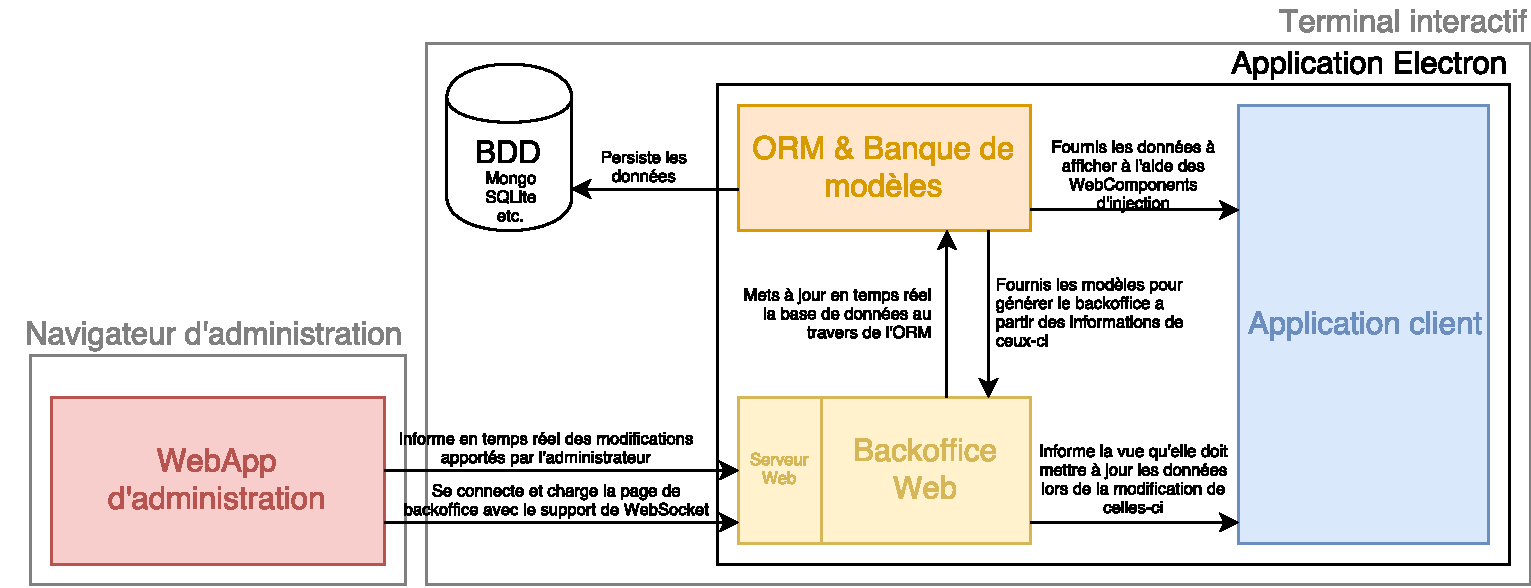
\includegraphics[scale=0.9]{Proposition-utopia.pdf}
        \caption{Structure général de l'application Biomérieux}
    \end{figure}
\end{landscape}

\clearpage

\subsubsection{Design}

Le design de cette application est fournis par le graphiste de vendredi 4 et se présente en une suite d'images représentant les différentes pages de l'application.
Ce design présente aussi une vidéo permettant de se représenter les différentes animations de l'application.

\begin{figure}[h]
    \centering
    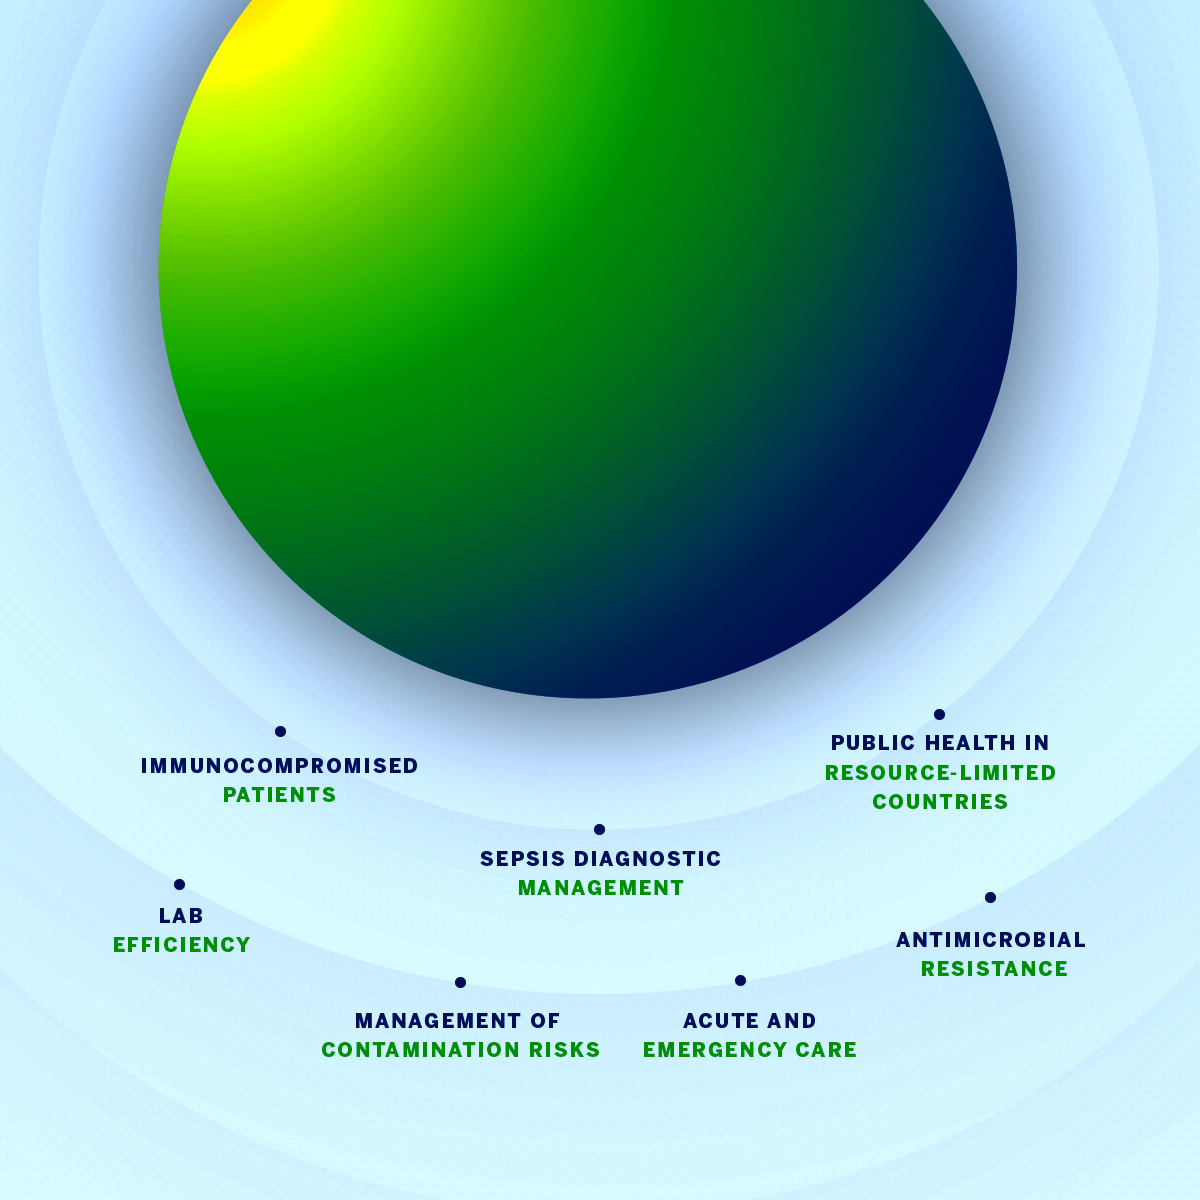
\includegraphics[scale=0.095]{bmx-1-initial.jpg}
    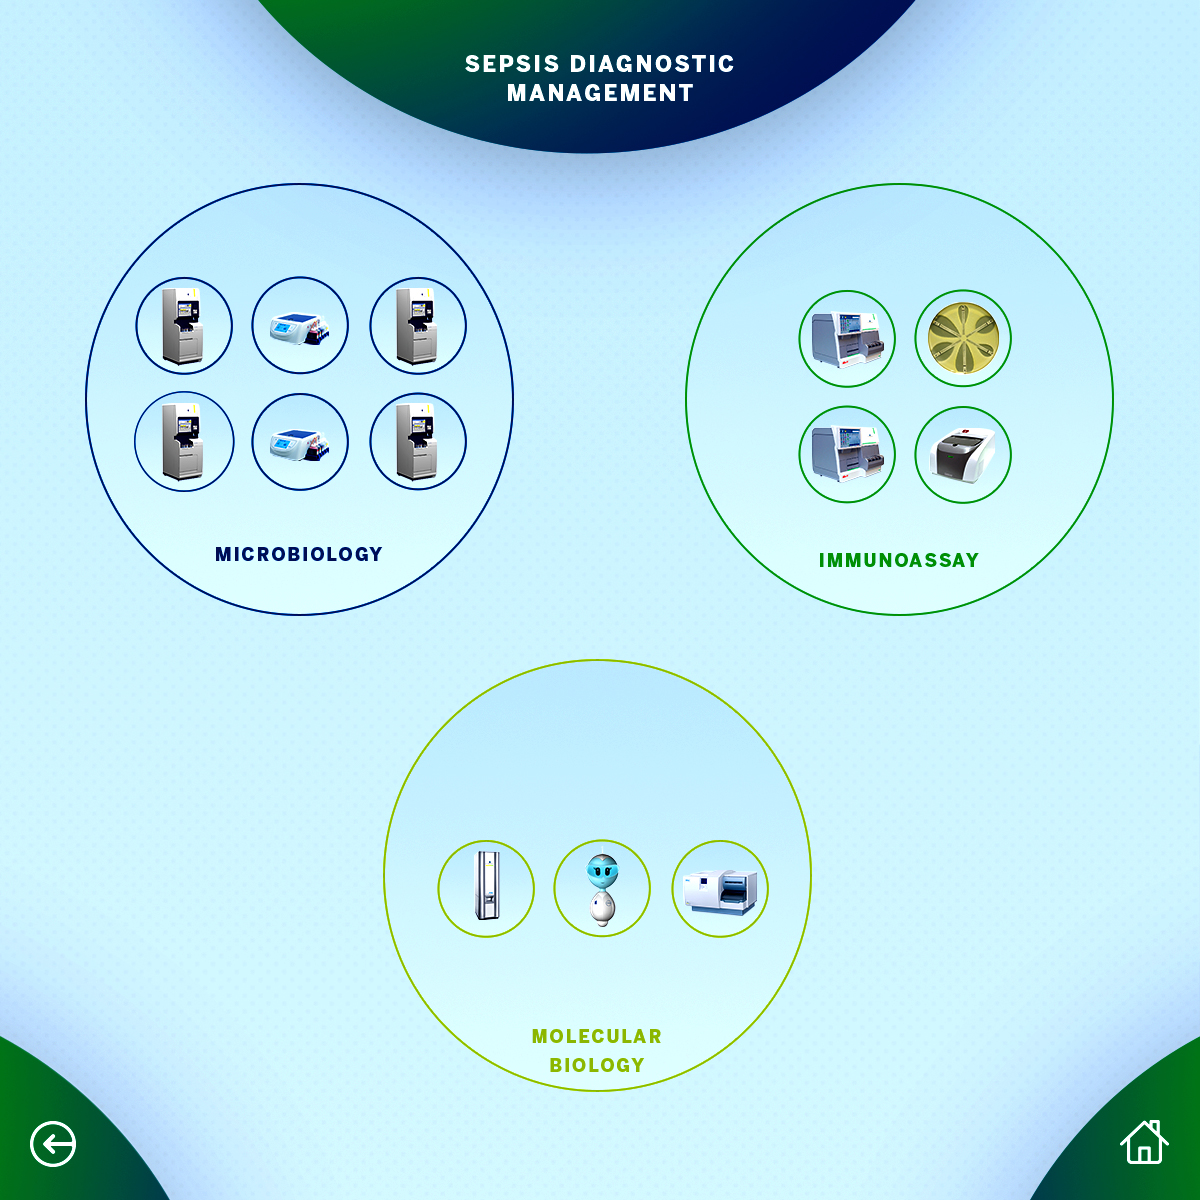
\includegraphics[scale=0.19]{bmx-2-initial.jpg}
    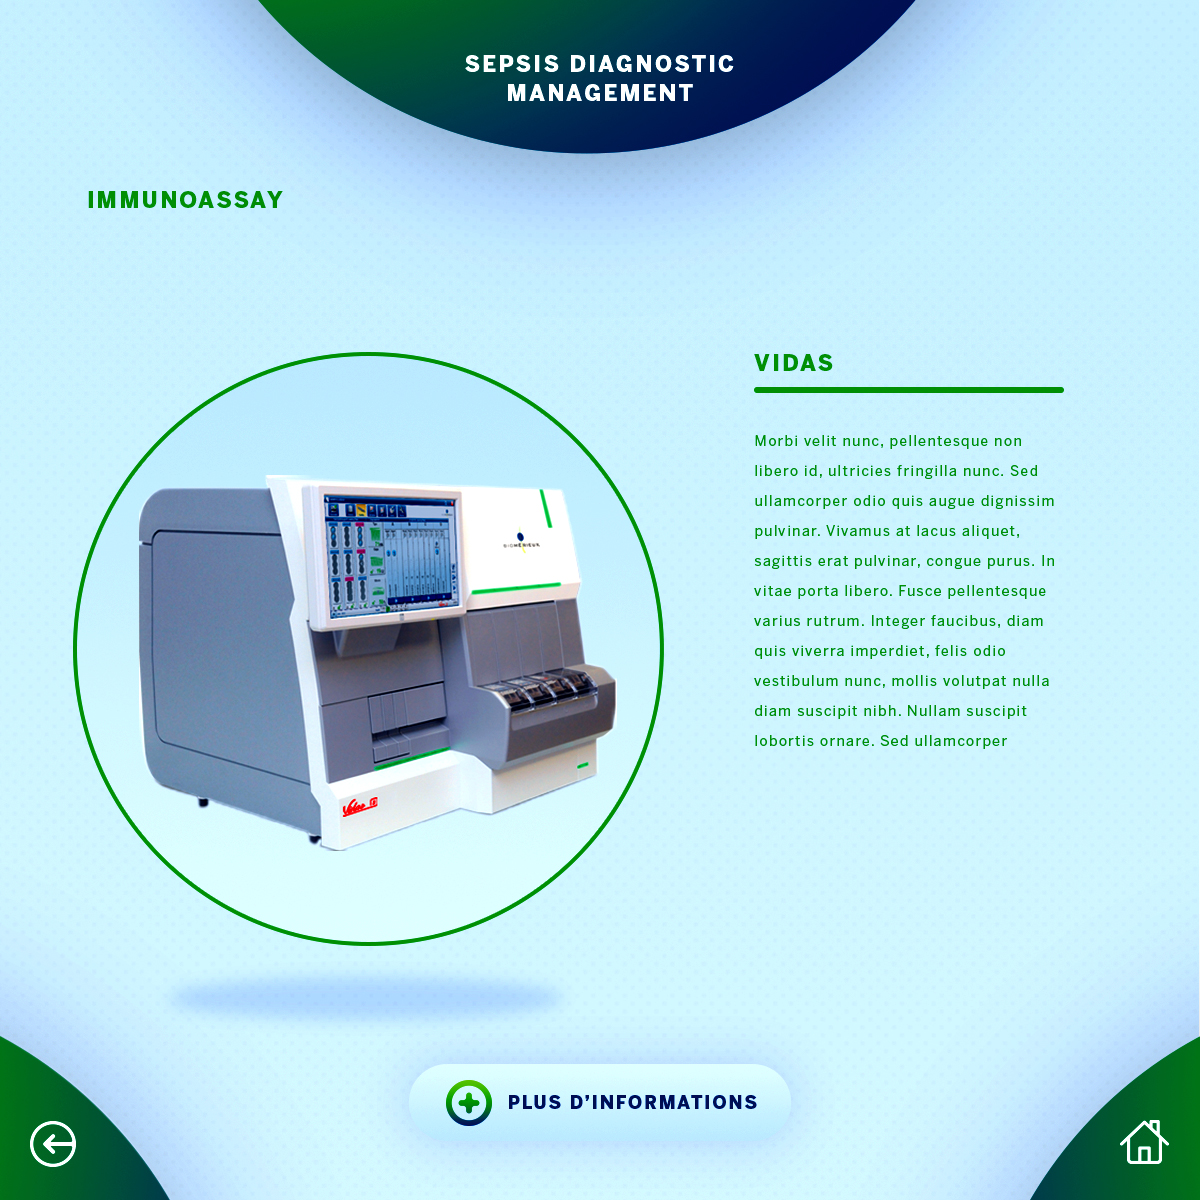
\includegraphics[scale=0.095]{bmx-3-initial.jpg}
    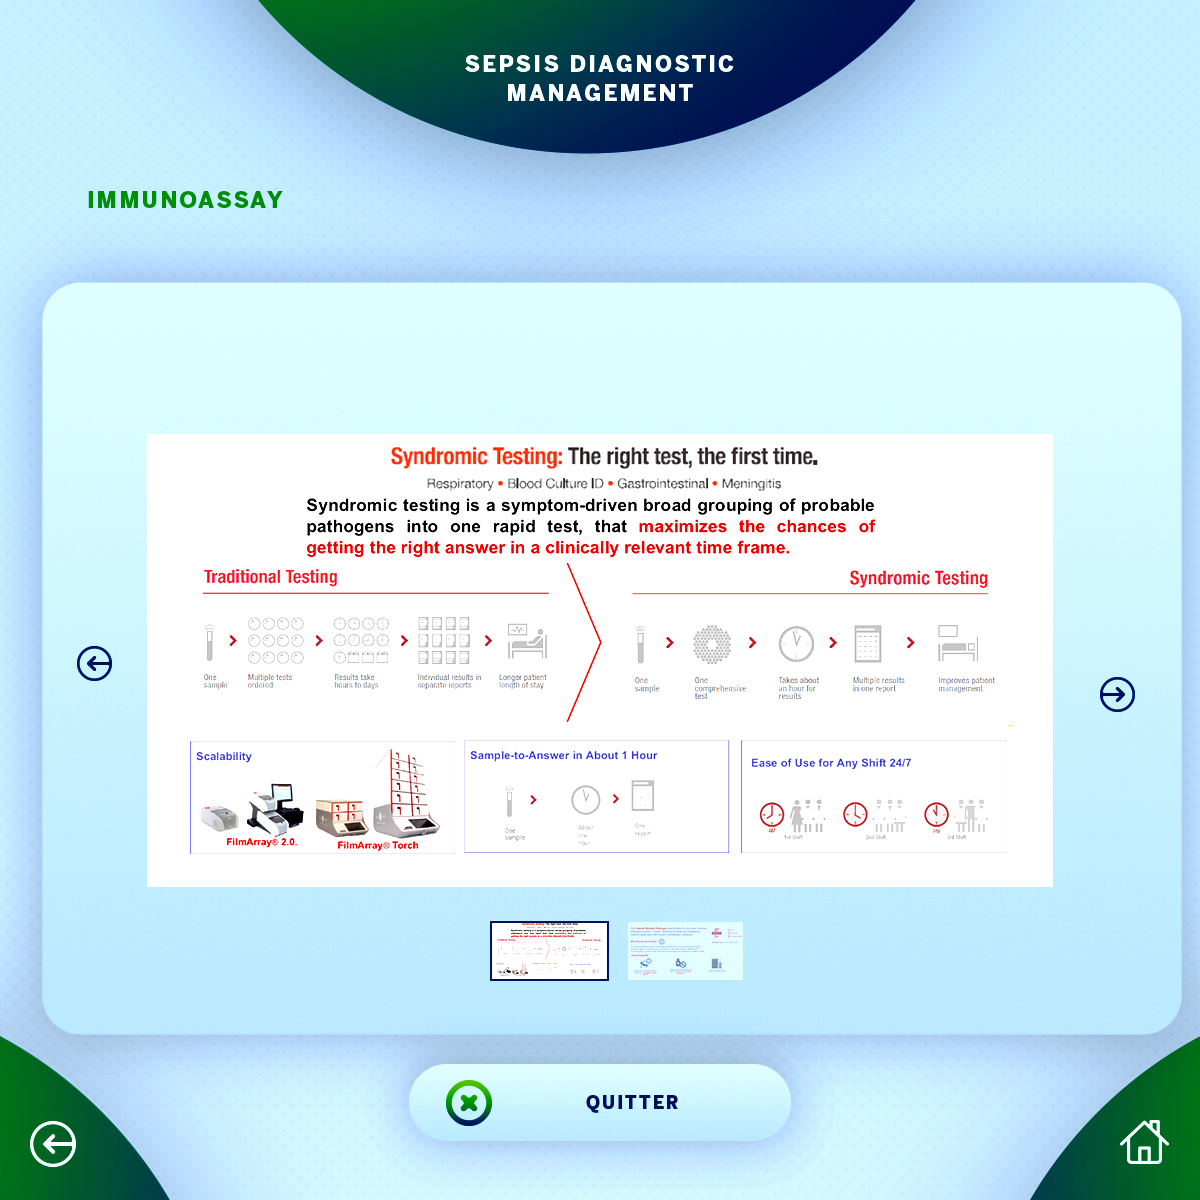
\includegraphics[scale=0.095]{bmx-4-initial.jpg}
    \caption{Design initial de l'application Biomérieux}
\end{figure}

Cependant, ce design à été fait en même temps que le remaniment de la charte graphique de la société.
Il en resulte que ce design ne correspond pas à la nouvelle charte graphique et qu'il fallait de remanier pour qu'il se plie aux nouvelles directives, nouveau logo et nouvelle palette de couleur.

\begin{figure}[h]
    \centering
    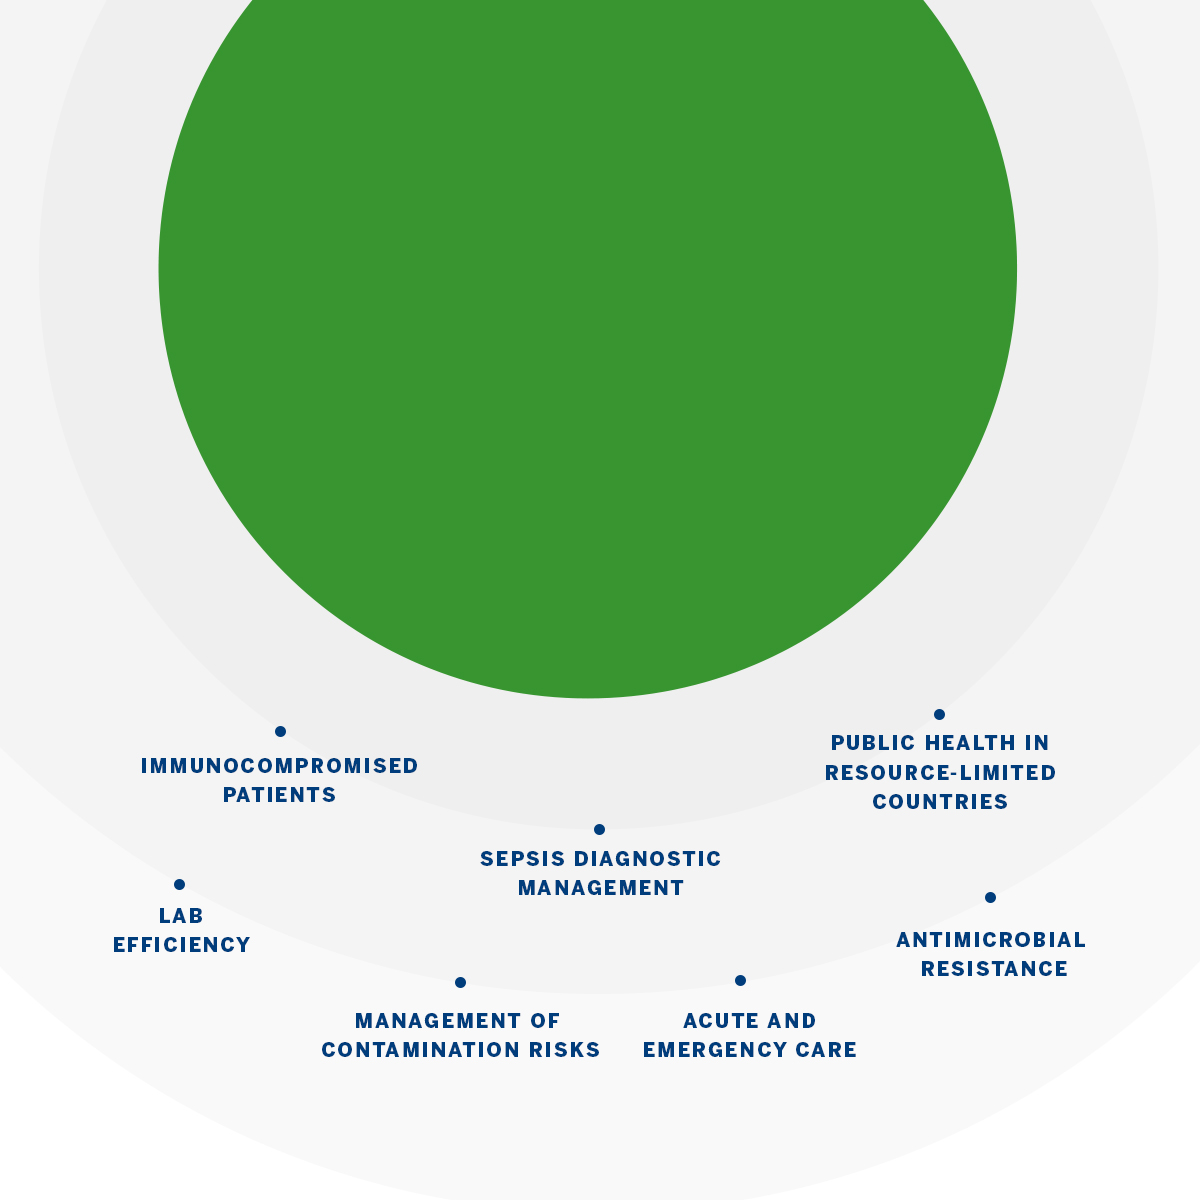
\includegraphics[scale=0.095]{bmx-1-new.jpg}
    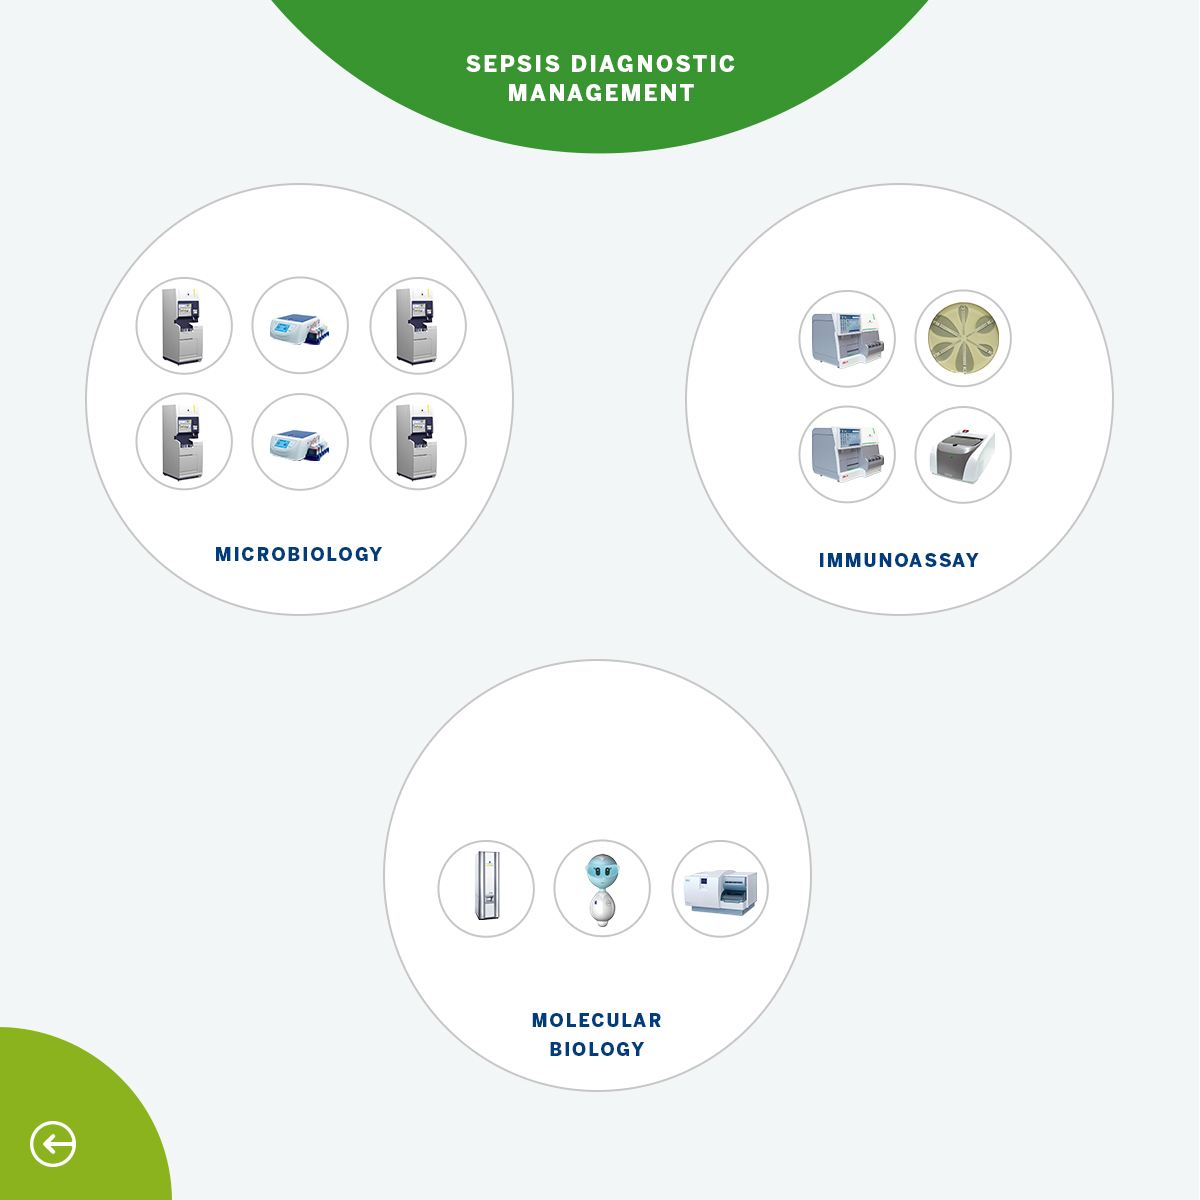
\includegraphics[scale=0.095]{bmx-2-new.jpg}
    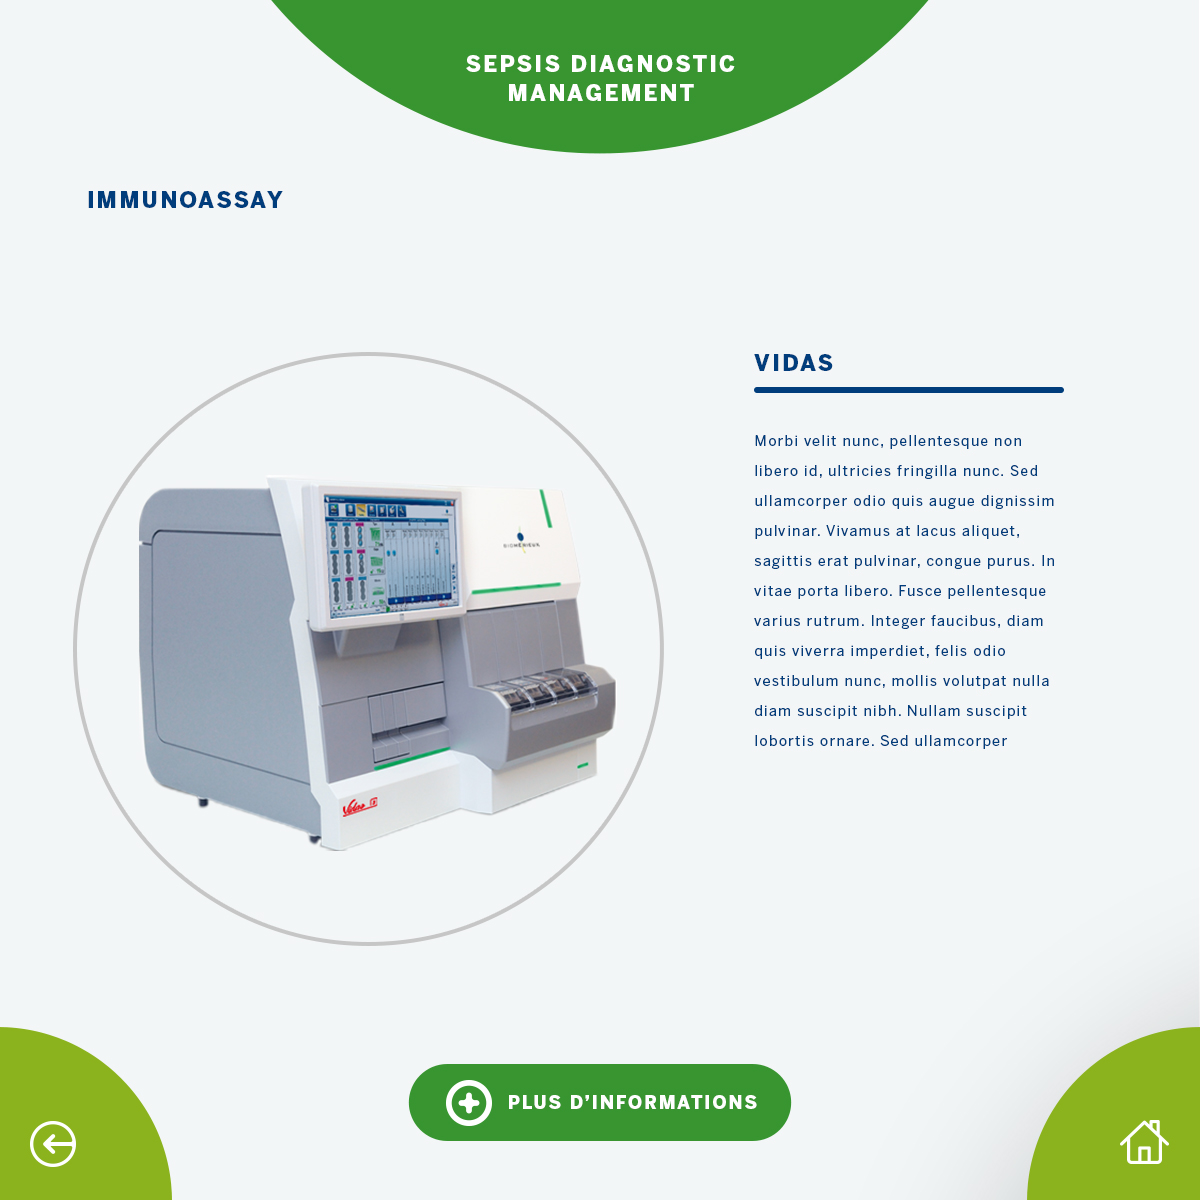
\includegraphics[scale=0.095]{bmx-3-new.jpg}
    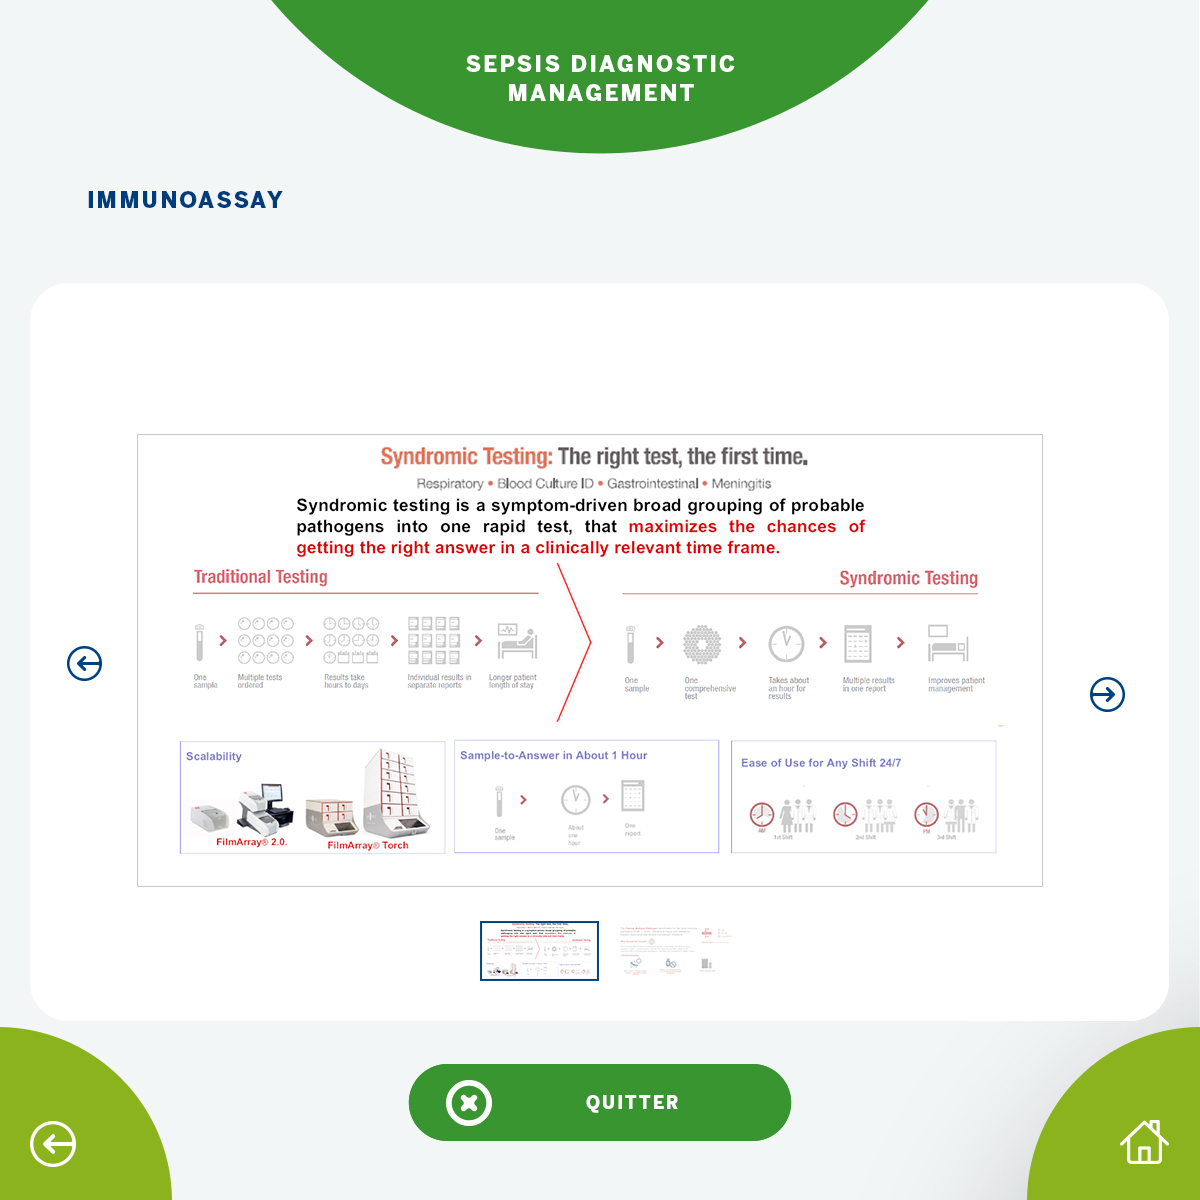
\includegraphics[scale=0.095]{bmx-4-new.jpg}
    \caption{Design renouvelé de l'application Biomérieux}
\end{figure}

\subsubsection{Conclusion}

Ce projet fut une bonne introduction aux techniques des WebComponents et à la manière de travailler des équipes LTBL.

Dans ce projet j'ai opté pour une strcture très classique ressemblant à un site Web.
Avec la recul, je me rend compte qu'il y a peut être une solution plus simple et plus flexible et que la solution que j'ai porposée demnde trop de création pour pas grand chose.
Par exemple, il n'est pas nécéssaire de penser les données en amont de l'application car, dans ce type d'installation, l'apparence finale prévaut sur le contenu.
On peut imaginer un système ou l'on arrange des WebComponents au lieu de générer l'interface sur la base de données.

Ce projet dure depuis 3 semaines et arriven bientot à son terme avec une première présentation au client le 7 férvier.

\subsection{Installation au salon de l'entreprise du futur}

Une partie du travaille chez LTBL passe par l'installation des systèmes développés chez le client.
J'ai eu l'occasion de participer à l'installation d'un projet d'ecran transparent au salon de l'entreprise du futur.

L'entreprise du futur est un collectif d'entreprise ayant pour objectif d'accompagner ces sentrprises dans la transformation numérique.
A l'occasion du salon de l'entreprise du futur à la cité international, LTBL à produit 4 ecrans transparents permettant de mettre en valeur un produit placé a l'interieur.
Le produit est alors entouré d'informations sur la société en question.

\begin{figure}[h]
    \centering
    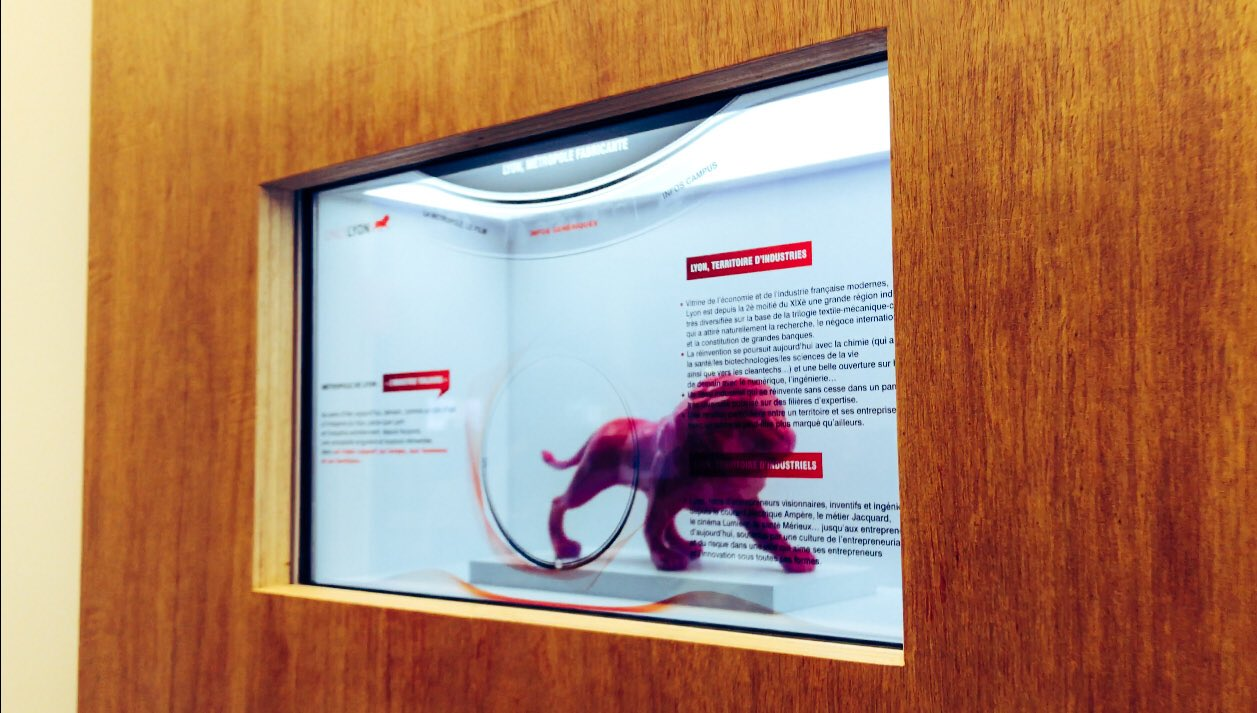
\includegraphics[scale=0.3]{ecran-transparent.jpg}
    \caption{Ecran transparent "Only Lyon" au salon de l'entreprise du futur}
\end{figure}

\subsubsection{Technologies}

Pour l'affichage, on utilise des ecrans transparents disposant d'une plaque a cristaux liqudes permettant d'afficher des informations et d'un compartiment uniformément éclairé en blanc permettant d'y placer un produit.
Sur cet écran s'affichent les informations sur le produit et des vidéos.

Pour afficher toutes ces informations, on utilise un mini ordinateur Asus VivoStick sous Windows 10 avec un site internet affiché en plein ecran avec Google Chrome.

Une enceinte USB est disposée au dessus de l'écran pour diffuser le son des vidéos.

\subsubsection{Conclusion}

Malgré que je n'ai pas travaillé sur ce projet, l'installation fut très interessant.
Je n'avais jamais fait ce type d'intervention et j'ai appris beacuoup de choses sur les éléments à mettre en place pour éviter tout problème.

\subsection{Blind Test}

\section{Missions à venir}

\section{Conclusion}

\section{Bilan}

\end{document}